\chapter{Sistemas lineales de primer orden}
\section{Introducción. Propiedades de estructura}
\begin{defi} Planteemos la formulación de un sistema lineal.

Sean $\alpha,\beta\in\R,\ t\in[\alpha,\beta]$, $n^2$ coeficientes $a_{ij}(t)$ con $a_{ij}\in\Cgot([\alpha,\beta];\K)$ con $\K=\R$ ó $\C$ y $1\leq i,j\leq n$.\\
Denotamos $A(t)=\big(a_{ij}(t)\big)_{1\leq i,j\leq n}$ a la matriz de coeficintes $a_{ij}$ continuas en $[\alpha,\beta]$\\
Sean $b_j\in \Cgot([\alpha,\beta];\K)$ con $1\leq n$, denotamos $B(t)=\begin{pmatrix}b_1(t)\\\vdots\\b_n(t)
\end{pmatrix}=\big( b_1(t)\hdots b_n(t)\big)^t$.

Por último, definimos nuestro sistema lineal de primer orden como $u'=A(t)u+B(t)$ donde $u=\begin{pmatrix}u_1\\\vdots\\u_n\end{pmatrix}=\big( u_1\hdots u_n\big)^t$ es una incógnita.
\end{defi}

\begin{defi} Decimos que $u\in\Cgot^1([\alpha,\beta];\K^n)$ es solución si $u_j\in\Cgot^1([\alpha,\beta];\K),\\
u_j'\in\Cgot([\alpha,\beta];\K)\ \forall 1\leq j\leq n$ y se cumple que:
\[u'(t)=A(t)u(t)+B(t)\ \forall t\in[\alpha,\beta]\]
Denotamos $\Sigma_B=\{u\in\Cgot^1([\alpha,\beta];\K^n)\ |\ u$ es solución de $u'=Au+B$ en $[\alpha,\beta]\}$.
\end{defi}

\begin{defi} Sea $u=A(t)u+B(t)$ un sistema de lineal de primer orden, definimos el \textbf{sistema homogéneo asociado} como $u'=A(t)u$ que puede ser representado como la función $f(t,u)=A(t)u$. Además, $f(t,\lambda u)=A(t)\lambda u=\lambda f(t,u)$. Denotamos\\
$\Sigma_0=\{h\in\Cgot^1([\alpha,\beta];\K^n)\ |\ h$ es solución de $u'=Au$ en $[\alpha,\beta]\}$
\end{defi}

\begin{proposicion} Propiedades de estructura.
\begin{enumerate}[1)]
\item Principio de superposición (o combinación lineal). Sean $h_1,h_2\in \Sigma_0, \lambda, \mu\in\K\implies\\\implies \lambda h_1(t)+\mu h_2(t)\in\Sigma_0$. Esto es, $\Sigma_0$ es una variedad vectorial $\Cgot^1(\alphabeta;\K)$.
\item Sean $u_1,u_2\in\Sigma_B$ entonces $u_1-u_2\in\Sigma_0$ y sean $h\in\Sigma_0$ y $u\in\Sigma_B$ entonces $u+h\in\Sigma_B$. Esto es, $\Sigma_B$ es una variedad afín en la dirección de $\Sigma_0$, es decir, paralela a $\Sigma_0$.
\end{enumerate}
\begin{proof}\ 
\begin{enumerate}[1)]
\item $(\lambda h_1+\mu h_2)'=\lambda h_1'+\mu h'2=\lambda Ah_1 + \mu Ah_2=A(\lambda h_1+\mu h_2)\implies(\lambda h_1+\mu h_2)\in\Sigma_0$
\item Tenemos $(u_1-u_2)'=u_1'-u_2'=(Au_1+B)-(Au_2+B)=A(u_1-u_2)\implies (u_1-u_2)\in\Sigma_0$.
Para acabar, $(u+h)'=u'+h'=Au+B+Ah=A(u+h)+B\implies (u+h)\in\Sigma_B$.
\end{enumerate}
\end{proof}
\end{proposicion}

\section{Ecuaciones lineales escalares}
\begin{defi} Sea una ecuación escalar, es decir, si el problema se trata en $n=1$, o sea en $\K$, tenemos: 
$\doubleleft{u'=a(t)u+b(t)\ \mathrm{con\ }a,b\in\Cgot([\alpha,\beta];\K)}{u(t_0)=u_0\in\K,\ t_0\in[\alpha,\beta]}$\\
A este problema lo denotamos como \textbf{problema de los valores iniciales} (P.V.I) o \textbf{problema de \textit{Cauchy}}.
\end{defi}


\begin{teor} Para cada $u_0\in\K$ y $t_0\in\alphabeta$, el P.V.I. $\doubleleft{u'=au+b}{u(t_0)=u_0}$ tiene una única solución y viene dada por $u(t;t_0,u_0)=e^{\inte{t}{t_0}a}u_0+\integral{t}{t_0} e^{\inte{t}{s}a}b(s)ds$.\\
\begin{proof}\ \\
Sea el problema homogéneo $h'=a(t)h$ entonces $h(t)=e^{\inte{t}{t_0}a}$, luego $h(t_0)=1$.
Sea $v(t)$ tal que $u(t):=h(t)v(t)$, esto es $\doubleleft{h'v+hv'=ahv+b\ximplies{h'v=ahv}{}hv'=b}{u_0=u(t_0)=h(t_0)v(t_0)\overset{h(t_0)=1}=v(t_0)}$ Tenemos además que $h^{-1}(t)=e^{-\inte{t}{t_0}a}$ luego $\doubleleft{v'(s)=b(s)e^{-\inte{t}{t_0}a}}{v(t_0)=u_0}$ con $s\in\alphabeta$ Por tanto,\\
$v(t)=\integral{t}{t_0}e^{-\inte{t}{t_0}a}b(s)ds+u_0$. Por último $u(t)=h(t)v(t)=e^{\inte{t}{t_0}a}\left(u_0+\integral{t}{t_0}e^{-\inte{s}{t_0}a}b(s)ds  \right)=$\\
$=e^{\inte{t}{t_0}a}u_0+\integral{t}{t_0}e^{\inte{t}{t_0}a-\inte{s}{t_0}a}b(s)ds\overset{\inte{t}{t_0}a=\inte{t}{s}a+\inte{s}{t_0}a}=e^{\inte{t}{t_0}a}u_0+\integral{t}{t_0}e^{\inte{t}{s}a}b(s)ds$.
\end{proof}
\end{teor}

\begin{defi} Al cambio de variable $u(t)=h(t)v(t)$ realizado en la demostración anterior y a su posterior desarrollo se le denomina \textbf{fórmula de la variación de los coeficientes de \textit{Lagrange}}.
\end{defi}

\begin{corolario} Entonces tenemos:\\
$(P)\doubleleft{u'=a(t)u+b(t)}{u(t_0)=u_0}$ tiene solución única y es $u(t;t_0,u_0)=e^{\inte{t}{t_0}a}u_0+\integral{t}{t_0}e^{\inte{t}{s}a}b(s)ds$\\
$(P_h)\doubleleft{u'=a(t)u}{u(t_0)=u_0)}$ tiene solución única y es $h(t;t_0,u_0)=e^{\inte{t}{t_0}a}u_0$

Observamos además que $u(t;t_0,0)=\integral{t}{t_0}e^{\inte{t}{s}a}b(s)ds$ es única solución de\\
$\doubleleft{u'=a(t)u+b(t)}{u(t_0)=0}$ de lo que se extrae que $u(t;t_0,u_0)=h(t;t_0,u_0)+u(t;u_0,0)$
\end{corolario}

\begin{teor}\ \begin{enumerate}[1)]
\item El operador solución $\xfunction{S_0}{\K}{\Sigma_0}{x\mapsto h(t;t_0, x)=e^{\inte{t}{t_0}a}x}$ es isomorfismo vectorial.
\item El operador solución $\xfunction{S_B}{\K}{\Sigma_B}{x\mapsto u(t;t_0, x)}$ es isomorfismo afín.
\end{enumerate}
En particular, $\dim\Sigma_0=\dim\Sigma_B=1$.
\begin{proof}\ 
\begin{enumerate}[1)]
\item Probemos la linealidad. Sean $x,y,\lambda,\mu\in\K,\ S_0(\lambda x+\mu y)= e^{\inte{t}{t_0}a}(\lambda x+\mu y)=\lambda e^{\inte{t}{t_0}a}x+\\+\mu e^{\inte{t}{t_0}a}y=\lambda S_0(x)+\mu S_0(y)$, luego es lineal. Tenemos además que\\
$S_0(x)=0\iff e^{\inte{t}{t_0}a}x=0\implies x=0$ luego $S_0$ es inyectiva.\\
Para acabar, si $h\in\Sigma_0$ tenemos que $h=h(t;t_0,h(t_0))=S_0(h(t_0)$ luego es sobreyectiva, y por tanto isomorfismo vectorial.
\item Tenemos que $S_B(x)=u(t;t_0,u_0)=h(t;t_0,u_0)+u(t;t_0,u_0)=S_0(x)+u(t;t_0,0)\in S_B$ es isomorfismo afín por ser un isomorfismo vectorial más un punto afín.
\end{enumerate}
\end{proof}
\end{teor}

\begin{observacion} Podemos observar que la variedad vectorial originada por una ecuación escalar $\Sigma_0=L\left[e^{\inte{t}{t_0}a}\right]$ y por tanto la solución general o conjunto de soluciones de $h'=a(t)h$ viene determinado por $e^{\inte{t}{t_0}a}x$ con $x\in\K$ lo que denominamos como ecuaciones paramétricas de $\Sigma_0$.\\

Por otro lado, el conjunto de soluciones de $\Sigma_B$ viene determinado por las ecuaciones paramétricas
$e^{\inte{t}{t_0}a}x+p(t)$ con $x\in\K$ y $p(t)$ cualquier solución de $\Sigma_B$, en particular podemos elegir $p(t)=u(t;t_0,0)$.
\end{observacion}

\begin{ejem} Sea $u'=au+b$ con $a,b\in \C$ ó $\R$\\
Tenemos como una solución particular $u=-\dfrac{b}{a}$ y solución de la homogénea $h'=ah$, $h=e^{at}$. Luego la solución general es $e^{at}x-\dfrac{b}{a}$.
\end{ejem}

\begin{ejem} Sea $\doubleleft{u'=au+b}{u(t_0)=u_0}$ con $a,b\in \C$ ó $\R$\\
Tenemos, por el ejemplo anterior, que la solución general de $u$ es $e^{at}x-\dfrac{b}{a}$, luego\\
$u_0=e^{at_0}-\dfrac{b}{a}\implies x = e^{-at_0}\left(u_0+\dfrac{b}{a}\right)$. Por lo que $u(t;t_0,u_0)=e^{at}e^{-at_0}\left(u_0+\dfrac{b}{a}\right)-\dfrac{b}{a}=\\=e^{a(t-t_0)}\left(u_0+\dfrac{b}{a}\right)-\dfrac{b}{a}$.
\end{ejem}

\begin{ejem}
Hagamos un ejemplo más específico. Sea  $u'=au+e^{wt}$, distingamos casos:
\begin{itemize}
\item Si $w\neq a$.\\
Sabemos que la solución del problema tendrá esta forma $e^{at}x + p(t)$ siendo $p(t)=me^{wt}$ una solución particular. Entonces metamos $p(t)$ en la ecuación y hallemos cuanto tiene que valer $m$. Luego $mwe^{wt}= ame^{wt} + e^{wt} \implies m(w-a)=1$ y despejando  $m=\dfrac{1}{w-a}$. 
Por tanto la solución general es $u(t)= e^{at}x + \dfrac{e^{wt}}{w-a}$.
\item Si $w=a$.\\
Entonces el sistema queda como $u'=au +e^{at}$. Para resolverlo en este caso variemos coeficientes. 
$u(t)=e^{at}v(t) \implies ae^{at}v(t) + e^{at}v'(t)= ae^{at}v(t)+e^{at} \implies e^{at}v'(t)=e^{at} \implies v'(t)=1 \implies v(t)=t + x$ con $x \in \C$. Por tanto la solución general es $u(t)=e^{at}x +te^{at}$. 
\end{itemize}
\end{ejem}

\begin{ejem} Sea $\doubleleft{u'=u+b(t)}{u(t_0)=u_0}$ con $b(t)=\doubleleft{1\ \mathrm{si}\ t\geq0}{0\ \mathrm{si}\ t<0}$.\\
En este caso observamos que la solución $u$ no puede ser una función de clase $\Cgot^1$ porque la derivada $u'$ no es continua ya que $b(t)$ no lo es. Veamos cual es la solución:\\
Aplicando la fórmula de la variación de las constantes, tenemos que \\ $u(t)= e^{t}u_0 + \inte{0}{t}e^{t-s}b(s)ds = \doubleleft{e^{t}u_0 + \inte{0}{t}e^{t-s}ds \ \mathrm{si}\ t>0}{e^{t}u_0 \ \mathrm{si}\ t<0}$ con lo que, calculando la integral, llegamos a que $u(t)=\doubleleft{e^{t}u_0 + e^{t}-1 \ si\ t>0}{e^{t}u_0 \ si\ t<0}$.\\
Obligamos a que la $u$ sea al menos continua ya que $u(0)=u_0$ por izquierda y derecha.
\end{ejem}

\begin{observacion} Observamos que si la función $a(t)$ en $u'=au + b$ no es  $\Cgot^1$ entonces no se puede garantizar la unicidad de la solución. Por ejemplo, sea:\\\\
$\doubleleft{u'=\dfrac{u}{t} }{u(0)=0}$ con $t \in \R \setminus\{0\}$. Tenemos que tanto $u_1=0$ y $u_2=t$ son soluciones del sistema.
\end{observacion}


\section{Teorema de unicidad}

\begin{lema}
Sea $u \in \Cgot(\alphabeta;\K^n)$ y sea $(P)=\doubleleft{u'=a(t)u +b(t)}{u(t_0)=u_0}$, entonces las siguientes afirmaciones son equivalentes.
\begin{enumerate}[1)]
\item $u \in \Cgot^1([\alpha,\beta];\K^n)$ y resuelve $(P)$.
\item $u(t)= u_0 + \inte{t_0}{t} a(s)u(s) +b(s) ds\ \forall t \in \alphabeta$. A esta ecuación se la denomina, ecuación integral asociada a $(P)$.
\end{enumerate}
\begin{proof}\ 
\begin{itemize}
\item $(1)\implies(2)$\\
Supongamos que se cumple $(1)$, entonces sabemos que $u$ resuelve $(P) \implies u'=\\
= A(t)u + B(t) \implies \inte{t_0}{t}u'(s)ds = \inte{t_0}{t}A(s)u(s) + B(s) ds \implies u(t)- u(t_0) =\\= \inte{t_0}{t}A(s)u(s) + B(s) ds \ximplies{u(t_0)=u_0}{} u(t)= u_0 + \inte{t_0}{t}A(s)u(s) + B(s) ds$.
\item $(2)\implies(1)$\\
Supongamos ahora que se cumple $(2)$, tenemos que $s \mapsto A(s)u(s)+B(s)$ es una función continua, luego $\dfrac{d}{dt}\inte{t_0}{t}A(s)u(s) + B(s)ds \overset{\mathrm{T.\ fund.\ c\acute{a}lculo}}= A(t)u(t)+B(t)$. Con lo que $u(t)\in \Cgot^1(\alphabeta;\K^n)$ ya que derivando la ecuación integral observamos que $\dfrac{d}{dt}u=\dfrac{d}{dt}u_0 + \dfrac{d}{dt}\inte{t_0}{t}A(s)u(s) + B(s)ds \implies u'(t)= A(t)u(t)+B(t)$. Esto nos da que $u'(t)$ es una función continua porque las otras 3 lo son, además $u(t_0)=u_0$ con lo que $u$ resuelve $(P)$.
\end{itemize}
\end{proof}  
\end{lema}

\begin{defi} Llamamos operador integral a $\xfunction{K}{\Cgot(\alphabeta;\K^n)}{\Cgot(\alphabeta;\K^n)}{h\mapsto u_0 + \inte{t_0}{t}A(s)h(s) + B(s)ds}$.

Podemos observar que $u(t)=u_0 + \inte{t_0}{t}\big(A(s)u(s) + B(s)\big)ds \implies u=Ku \iff u$ es un punto fijo de $K$.
\end{defi}

\begin{defi} Sea $u\in\Cgot([\alphabeta];\K^n)$ con norma $\norm{\cdot}$, definimos la norma infinito $\norm{u}_\infty=\underset{t\in[\alphabeta]}\max\norm{u(t)}$. Además, tenemos que $\xfunction{f}{\Cgot([\alphabeta];\K^n)}{\R}{t\mapsto\norm{u(t)}}$ es continua y que:
\begin{enumerate}[1)]
\item $\norminf{u}\geq 0\ \forall u\in \Cgot(\alphabeta;\K^n)$. Además. $\norminf{u}=0\iff u=0$.
\item $\norminf{\lambda u}=|\lambda|\norminf{u}\ \forall u\in\Cgot(\alphabeta;\K^n),\ \forall \lambda\in\K$.
\item $\norminf{u_1+u_2}\leq\norminf{u_1}+\norminf{u_2}\ \forall u_1,u_2\in\Cgot(\alphabeta;\K^n)$.
\end{enumerate}
\end{defi}

\begin{defi} Definimos espacio de \textit{Banach} al espacio vectorial normado de funciones
$\big(\Cgot(\alphabeta;\K^n),\norm{\cdot}\infty\big)$.

Denotaremos como $X =(\Cgot(\alphabeta;\K^n),\norm{\cdot}_\infty)$ a dicho espacio de \textit{Banach}.
\end{defi}

\begin{proposicion} Sea $X$ espacio de \textit{Banach}, entonces es de dimensión infinita.
\begin{proof}
Sea $e\in\K^n$, con $e\neq 0$ y sea $t^ne,\ n\geq 0\y t\in\alphabeta$.\\
Si $c_0e+c_1te+c_2t^2e+...+c_nt^ne=0\iff e\stackbin[i=0]{n}\sum c_it^i=0$ para ciertos $c_i$. Como $e\neq0\implies\\
\implies \stackbin[i=0]{n}\sum c_it^i=0\implies \left(\stackbin[i=0]{n}\sum c_it^i\right)^{n)}=0\implies c_nn!=0\implies c_n=0\implies\\\implies \stackbin[i=0]{n-1}\sum c_it^i=0\ximplies{\mathrm{por\ recursi\acute{o}n}}{}=c_i=0\ \forall1\leq i\leq n\implies \{e,te,...,t^ne\}$ son linealmente independientes.
\end{proof}
\end{proposicion}

\begin{proposicion} Sea $X$ es un espacio de \textit{Banach}, entonces es completo; Es decir, cualquier sucesión de \textit{Cauchy} es convergente.
\begin{proof}\ \\
Sea $\{u_n \}_{n\geq 1}$ de Cauchy en $X$ entonces $\forall \varepsilon >0 \ \exists n_0 \in \N$ tal que $ \norminf{u_{n+m}-u_n} \leq\varepsilon \  \forall n \geq n_0$ y $m\geq1$.\\
$X$ es completo, si $\exists u \in X$  tal que $\limite{}{\ntiende}{u_n}=u$ en $X\iff\limite{}{\ntiende}{\norminf{u_n-u}}=0$.\\
Entonces, si $\norm{u_{n+m}-u_n}_\infty\leq \varepsilon \implies \norm{u_{n+m}(t)-u_n(t)} \leq  
\varepsilon \ \forall n \geq n_0( \varepsilon ) \ m \geq 1,\\
t \in \alphabeta \implies \{u_n(t)\}_{n\geq 1}$ es de Cauchy $\forall t \in \alphabeta$. Por tanto
como $\{u_n(t)\}_{n\geq 1}$ viven en $\K^n$ y sabemos que $\K^n$ es completo, entonces podemos asegurar que todas esas sucesiones son convergentes porque son de Cauchy en un espacio completo. 
Por lo que $\exists \lim_{\ntiende}{u_n(t)}=\\
=u(t) \implies \norm{u(t)-u_n(t)}_\infty\leq \varepsilon \ n\geq n_0 \ t \in \alphabeta$.

Veamos ahora que $u$ es continua y así la convergencia es uniforme. Observemos que:\\
$\norm{u(t+h)-u(t)} \leq \norm{u(t+h)-u_{n_0}(t+h)} + \norm{u_{n_0}(t+h)-u_{n_0}(t)} + \norm{u_{n_0}(t)-u(t)} \leq\\
\leq2\varepsilon+\norm{u_{n_0}(t+h)-u_{n_0}(t)}\leq 3\varepsilon$ para un cierto $t,t+h\in\alphabeta$ y cogiendo un\\
$|h|\leq \delta$ siendo $\delta$ de la continuidad uniforme en compactos de las funciones $u_{n_0}$.
Entonces $u$ es continua y además uniformemente continua ya que $\alphabeta$ es un compacto. 
Por tanto $\norminf{u-u_n} \leq\varepsilon$, con $\ n\geq n_0$, con lo que $\limite{}{\ntiende}{u_n-u}=0 \iff u_n\limited{u}$ en\\
$X =(\Cgot(\alphabeta;\K^n),\norm{\cdot}_\infty)$. Con lo que $X$ es completo.
\end{proof}
En la siguiente figura podemos ver un esquema de la aproximación de $u_n$ a $u$.
\begin{figura}\ \begin{center}\definecolor{zzttqq}{rgb}{0.6,0.2,0.}
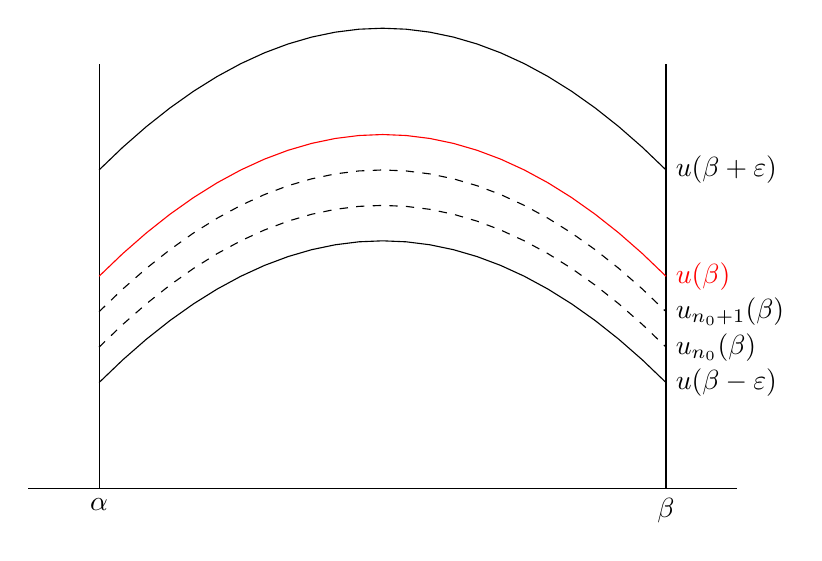
\begin{tikzpicture}[x=0.9cm,y=0.9cm]
\draw[color=black] (-1,0) -- (9,0);
\draw[color=black] (0,0) -- (0,6);
\draw[color=black] (8,0) -- (8,6);
\draw [domain=0:8, color=red] plot(\x,{-(1/8)*\x*\x+\x+3});
\draw [domain=0:8] plot(\x,{-(1/8)*\x*\x+\x+4.5});
\draw [domain=0:8] plot(\x,{-(1/8)*\x*\x+\x+1.5});
\draw [domain=0:8, dashed] plot(\x,{-(1/8)*\x*\x+\x+2.5});
\draw [domain=0:8, dashed] plot(\x,{-(1/8)*\x*\x+\x+2});
\draw[color=red] (8,3) node[anchor=west] {$u(\beta)$};
\draw (8,4.5) node[anchor=west] {$u(\beta+\varepsilon)$};
\draw (8,1.5) node[anchor=west] {$u(\beta-\varepsilon)$};
\draw (8,2) node[anchor=west] {$u_{n_0}(\beta)$};
\draw (8,2.5) node[anchor=west] {$u_{n_0+1}(\beta)$};
\draw (0,0) node[anchor=north] {$\alpha$};
\draw (8,0) node[anchor=north] {$\beta$};


\end{tikzpicture}\end{center}\end{figura}

\end{proposicion}

\begin{defi}
Sea $u\in X$ con $X$ el espacio de Banach definido anteriormente. Definimos la norma Bielecky $\norm{u}_B=\underset{t\in\alphabeta}\max\{\e^{-B|t-t_0|}\norm{u(t)}\}$ para un $B>0$ y un $t_0 \in \alphabeta$.
\end{defi}

\begin{observacion}Las dos normas que hemos defnido, la norma infinito $\norm{\cdot}_\infty$ y la norma Bielecky $\norm{\cdot}_B$ son equivalentes. Para verlo basta comprobar que $\norm{\cdot}_B \leq \norm{\cdot}_\infty \leq \e^{(\beta - \alpha)}\norm{\cdot}_B$
\end{observacion}

\begin{teor} Teorema de la aplicación contractiva.\\
Sea $X$ espacio de Banach, y sea $\function{K}{X}{X}$ tal que $\norm{Kx-Ky} \leq \theta\norm{x-y} \\
\forall x,y \in X, \theta \in [0,1)$ entonces $\exists! x^* \in X$ tal que $Kx^*=x^*$.\\
Además para cada $x_0 \in X$ el esquema iterativo $x_n=Kx_{n-1}$ para $ n\geq 1$, converge a $x^{*}$.\\
La prueba de este teorema fue vista en la asignatura de \textit{Cálculo diferencial}.
\end{teor}

\begin{teor} Teorema de la solución única.\\
Sean $a_{ij},b_j\in\Cgot(\alphabeta;\K)\y A=\big(a_{ij}\big)_{1\leq i,j\leq n}, B=(b_j)_{1\leq j\leq n}$, entonces $\forall t_0\in\alphabeta\y u_0\in\K^n$, el problema de valores iniciales $\doubleleft{u'=A(t)u+B(t)}{u(t_0)=u_0}$ tiene una única solución en $\alphabeta$.
\begin{proof} \ \\
Sea $\xfunction{K}{\Cgot(\alphabeta;\K^n)}{\Cgot(\alphabeta;\K^n)}{h\mapsto u_0+\inte{t}{t_0}\big(A(s)h(s)+B(s)\big)ds}$, probemos que es contractiva; Es decir, probemos que\\
$\normbi{Ku-Kv}\leq\theta\normbi{u-v}$ con $\theta\in(0,1)$.\\
Tenemos $e^{-B|t-t_0|}\norm{Ku(t)-Kv(t)}\overset{\norm{x}\leq C_1\norm{x}_1}\leq C_1 e^{-B|t-t_0|}\norm{Ku(t)-Kv(t)}_1=\\
=e^{-B|t-t_0|}\norm{\integral{t}{t_o}A(s)\big(u(s)-v(s)\big)ds}_1(*)$.\\

Por otro lado, $\norm{\integral{t}{t_0}\begin{pmatrix}x_1(s)\\\vdots\\x_n(s)\end{pmatrix}ds}_1=\stackbin[j=1]{n}\sum\left|\integral{t}{t_0}x_j(s)ds\right|\leq \stackbin[j=1]{n}\sum\integral{\max\{t,t_0\}}{\min\{t,t_0\}}\left|x_j(s)\right|ds=\\
=\integral{\max\{t,t_0\}}{\min\{t,t_0\}}\stackbin[j=1]{n}\sum\left|x_j(s)\right|ds=\integral{\max\{t,t_0\}}{\min\{t,t_0\}}\norm{\begin{pmatrix}x_1(s)\\\vdots\\x_n(s)\end{pmatrix}}_1ds$.\\

Luego tenemos que $(*)\leq C_1e^{-B|t-t_0|}\integral{\max\{t,t_0\}}{\min\{t,t_0\}}\norm{A(s)\big(u(s)-v(s)\big)}_1ds\leq\\
\overset{\norm{x}\leq C_2\norm{x}_1}\leq C_1C_2e^{-B|t-t_0|}\integral{\max\{t,t_0\}}{\min\{t,t_0\}}\norm{A(s)\big(u(s)-v(s)\big)}ds(**)$.

\begin{nota} Hagamos una pausa para recordar la norma de una matriz.\\
Sea $A\in\mathfrak{M}_n(\K)\sim\K^{n^2}\sim\mathfrak{L}(\K^n)$, definimos norma de $A$ como:\\
$\norm{A}=\norm{A}_{\mathfrak{L}(K^n)}=\max\{\norm{Ax}:\norm{x}=1\}$. De aquí obtenemos que $\norm{Ax}=\norm{\norm{x}A\dfrac{x}{\norm{x}}}=\\
=\norm{x}\norm{A\dfrac{x}{\norm{x}}}\leq \norm{A}\norm{x}\ \forall x\in\K^n$.
\end{nota}
Por esto último $(**)\leq C_1C_2e^{-B|t-t_0|}\integral{\max\{t,t_0\}}{\min\{t,t_0\}}\norm{A(s)}_{\mathfrak{L}(K^n)}\norm{u(s)-v(s)}ds(***)$\\
Ahora tenemos que $\norm{A(s)}_{\mathfrak{L}(K^n)}\leq C_3\norm{A(s)}_1=C_3\stackbin[i,j=1]{n}\sum|a_{ij}(s)|\leq C_3\stackbin[i,j=1]{n}\sum\norminf{a_{ij}}$. Luego\\
$(***)\leq \boxed{C_1C_2C_3\stackbin[i,j=1]{n}\sum\norminf{a_{ij}}}_{\ =L}e^{-B|t-t_0|}\integral{\max\{t,t_0\}}{\min\{t,t_0\}}\norm{u(s)-v(s)}ds=\\
=Le^{-B|t-t_0|}\integral{\max\{t,t_0\}}{\min\{t,t_0\}}e^{B|s-t_0|}e^{-B|s-t_0|}\norm{u(s)-v(s)}ds\leq\\ Le^{-B|t-t_0|}\integral{\max\{t,t_0\}}{\min\{t,t_0\}}e^{B|s-t_0|}ds\normbi{u-v}(****)$. Finalizando tenemos:\\
Si $t>t_0$, entonces $\integral{\max\{t,t_0\}}{\min\{t,t_0\}}e^{B|s-t_0|}ds=\integral{t}{t_0}e^{B(s-t_0)}ds=\dfrac{e^{B(t-t_0)}-1}{B}=\dfrac{e^{B|t-t_0|}-1}{B}$.\\
Si $t<t_0$, entonces $\integral{\max\{t,t_0\}}{\min\{t,t_0\}}e^{B|s-t_0|}ds=\integral{t_0}{t}e^{-B(s-t_0)}ds=\dfrac{e^{-B(t-t_0)}-1}{B}=\dfrac{e^{B|t-t_0|}-1}{B}$.\\
De forma que $(****)=Le^{-B|t-t_0|}\dfrac{e^{B|t-t_0|}-1}{B}\normbi{u-v}\leq Le^{-B|t-t_0|}\dfrac{e^{B|t-t_0|}}{B}\normbi{u-v}=\\=\dfrac{L}{B}\normbi{u-v}$. Luego $\normbi{Ku-Kv}\leq\theta\normbi{u-v}$ con $\theta = \dfrac{L}{B}$ tomando $B>L$.
\end{proof}
\end{teor}

\begin{corolario} Iteraciones de \textit{Picard-Lindelöf}.\\
Para cualquier $h_0\in\Cgot(\alphabeta;\K^n)$, el esquema iterativo $h_n=Kh_{n-1}=K^nh_0$ con $n\geq 1$, es decir, $(h_0,Kh_0,K^2h_0...)$ converge a una única solución de $\doubleleft{u'=A(t)u+B(t)}{u(t_0)=u_0}$.
\end{corolario}

\begin{ejem} Sea $\doubleleft{h'=h}{u(t_0)=u_0}$ entonces $Kh(t)=u_0+\integral{t}{t_0}h(s)ds$.\\
Sea $h_0\equiv u_0$ (cte.), tenemos:\\
$h_1(t)=Kh_0(t)=u_0+\integral{t}{t_0}h_0(s)ds=u_0+u_0(t-t_0)=u_0(1+t-t_0)$.
$h_2(t)=Kh_1(t)=u_0+\integral{t}{t_0}u_0(1+s-t_0)ds= u_0(1+t-t_0+\dfrac{(t-t_0)^2}{2})$. $h_3(t)=Kh_2(t)= u_0 +\integral{t}{t_0}u_0(1+s-t_0+ \dfrac{(s-t_0)^2}{2})ds=u_0(1+t-t_0+ \dfrac{(t-t_0)^2}{2}) + \dfrac{(t-t_0)^3}{3!})$. Entonces $h_n(t)=u_0(1+t-t_0+ \dfrac{(t-t_0)^2}{2}) + \dfrac{(t-t_0)^3}{3!} + ... + \dfrac{(t-t_0)^n}{n!})\limited{\e^{(t-t_0)}u_0}$ de manera uniforme en $\alphabeta$.
\end{ejem}

\begin{corolario}
Bajo las condiciones del teorema fundamental, el operador solución $\xfunction{S_0}{\K^n}{\Sigma_0}{x\mapsto S_0(x)= h(t;t_0, x)}$, que determina una única solucion de $\doubleleft{h'=A(t)h}{h(t_0)=x}$, es isomorfismo vectorial.\\
Por tanto, el operador solución $\xfunction{S_B}{\K^n}{\Sigma_B}{x\mapsto S_B(x)=u(t;t_0, x)}$, que determina una única solucion de $\doubleleft{u'=A(t)u + B(t)}{u(t_0)=x}$, es isomorfismo afín.
Por ello, $\dim\Sigma_0=\dim\Sigma_B=n$. Además puesto que $S_0$ envía bases de $\K^n$ en bases de $\Sigma_0$, si $\K^n$ está generado por $(e_1,...,e_n) \implies \Sigma_0=L[h(t;t_0,e_1),...,h(t;t_0,e_n)]$.
\begin{proof}\ \\
Comprobemos que $S_0$ es lineal.

Sea $\lambda , \mu \in \K, \ x,y \in \K^n$. Entonces, $ S_0(\lambda x +\mu y)= h(t;t_0,\lambda x +\mu y)= \lambda h(t;t_0,x)+\\+ \mu h(t;t_0,y)= \lambda S_0(x) + \mu S_0(y)$.
Veamos que es inyectiva.

$S_0(x)=0 \implies x=h(t;t_0,x)=0 \implies x=0$. Además $S_0(x)=S_0(y) \iff\\\iff S_0(x-y)=0 \iff x=y$. También es fácil comprobar que es suprayectiva. En efecto:

Si $h \in \Sigma_0,\ h(t)=h\big(t;t_0,h(t_0)\big)$, por el \textit{Teorema de unicidad} $!\exists h(t)=S_0(h(t_0))$.\\
Luego $S_0$ es isomorfismo vectorial y $\dim\K^n = \dim \Sigma_0 = n$.
\end{proof} 
\end{corolario}

\section{Variación de coeficientes}

\begin{defi}
Diremos que $\Phi(t) = \begin{pmatrix}
h_{11}(t) & \hdots & h_{1n}(t) \\
\vdots & \ddots & \vdots \\
h_{n1}(t) & \hdots & h_{nn}(t)
\end{pmatrix}$ es una matriz de soluciones de $h' = A(t)h$ cuando sus columnas resuelven $h' = A(t)h$ es decir $\Phi'(t)= (h'_{ij}(t))= \begin{pmatrix} h_1'(t) \hdots	 h_n'(t) \end{pmatrix} = \begin{pmatrix} A(t)h_1(t) \hdots A(t)h_n(t) \end{pmatrix}= A(t)\begin{pmatrix} h_1(t) \hdots h_n(t) \end{pmatrix}=A(t)\Phi(t)$ o lo que es lo mismo, $\Phi(t)$ resuelve el sistema.
\end{defi}

\begin{defi}
$\Phi(t)$ es una matriz fundamental de soluciones (M.F.S.) cuando sus columnas son una base de $\Sigma_0$.
\end{defi}

\begin{ejem}
Sea $h'=Ah$ entonces $\Phi(t)= \e^{At}=\stackbin[n=0]{\infty}\sum\dfrac{A^nt^n}{n!}$ es una matriz fundamental de soluciones.
\end{ejem}

\begin{teor}
Sean $h_1,\hdots,h_n \in \Sigma_0$ y sea $\Phi=\begin{pmatrix} h_1 \hdots h_n \end{pmatrix}$. Entonces las siguientes afirmaciones son equivalentes:
\begin{enumerate}[1.]
\item $\Phi(t)$ es M.F.S. $\big(\Sigma_0 = L[h_1,..., h_n]\big)$.
\item $\exists t_0 \in \alphabeta$ tal que $\det\Phi(t_0)\neq 0$.
\item $\det\Phi(t)\neq 0 \ \forall t \in \alphabeta$.
\end{enumerate}
\begin{proof}\ \\
Supongamos que $\exists t_0 \in \alphabeta$ tal que $\det\Phi(t_0)=0 \implies \exists c_1,\hdots,c_n \in \K$ tal que\\
$c_1h_1(t_0)+c_2h_2(t_0)+ ... + c_nh_n(t_0)=0$ con $(c_1,...,c_n)\neq(0,...,0)$. Por tanto, sea\\
$h(t)=c_1h_1(t_0)+c_2h_2(t_0)+ \hdots + c_nh_n(t_0)=0 \ \forall t \in \alphabeta$, $h \in \Sigma_0$ y $h(t_0)=0 \implies\\
\implies h=0 \implies \{h_1,\hdots,h_n\}$ es linealmente dependiente (esto prueba, por contrarrecíproco, que $(1)\implies (3)$). Por lo que $\det\Phi(t)=0 \ \forall t \in \alphabeta$ ($(2)\implies(1)$). Para acabar, es evidente que ($(3)\implies(2)$).
\end{proof}
\end{teor}

\begin{proposicion}
El determinante de una M.F.S. $\Phi$ viene también determinado por la fórmula de Jacobi-Louiville: $\det\Phi(t)=\e^{\inte{t}{t_0}tr(A(s))ds}det\Phi(t_0)$ con $t,t_0 \in \alphabeta$. Es decir, obtenemos cualquier determinante de $\Phi(t)$, $t\in\alphabeta$ dado el valor del determinante de un punto $t_0$ cualquiera.
\end{proposicion}

\begin{observacion}
Hallemos la solución general de $u'= A(t)u(t) + B(t)$.
Sea $\Phi(t)=\begin{pmatrix} h_1 & \hdots & h_n \end{pmatrix}$ 

\end{observacion}

